\documentclass[12pt]{article}
\usepackage{graphicx} % Use this package to include images
\usepackage{amsmath} % A library of many standard math expressions
\usepackage[margin=1in]{geometry}% Sets 1in margins.
\usepackage{fancyhdr} % Creates headers and footers
\usepackage{enumerate}  %These two package give custom labels to a list
\usepackage{enumitem}
\usepackage{amssymb}
\usepackage{amsthm} % for theorem style environments for question and answers for readablity
\usepackage{titlesec}
% Customize section font size
\titleformat*{\section}{\fontsize{14pt}{16pt}\bfseries\selectfont}
% Customize subsection font size
\titleformat*{\subsection}{\fontsize{12pt}{14pt}\bfseries\selectfont}
\titlespacing*{\section}{0pt}{1ex}{0.5ex}
\titlespacing*{\subsection}{0pt}{0.8ex}{0.4ex}
\newtheorem*{thm}{Theorem}
\theoremstyle{definition}
\newtheorem*{q}{Question}
\newtheorem*{ans}{Answer}
\title{Naive Bayes Classifier Project Report}
\author{Garrett Nix}
\date{\today}
\begin{document}
\maketitle
\vspace{-2em}  % Remove space after title block
\section{Introduction}
In this assignment, concepts learned from class, specifically the implementation of a Naive Bayes model, is investigated.
The task of observing the performance of a Naive Bayes classifier as the training size increases is performed on bank data obtained from the UCI Machine Learning Repository. 
A table measuring this performance is discussed.

\section{Methodology}
The data obtained for this project is based on bank data obtained from the University of California Irvine Machine Learning Repository.
This data consists largely of categorical and binary features, having only 6 out of the 16 features being numerical. Loading the data into a dataframe in Python using the Pandas library, 
a delimeter set to `;' allowed for simple manipulation and functionality for data preprocessing. This preprocessing consists of one-hot encoding the categorical and binary columns into numerical values using the $\texttt{pd.get\_dummies()}$ method with the encoding data type set to integer. Indices having values as ``unknown''', these are removed as from a application standpoint, this could be used to provide more concise predictions in understanding the marketing demographics.

\section{Results}
Once this preprocessing was completed, the assignment was followed for each of the training/test splits specified fed into a NB classifier. Gathering the various averages and standard deviations for both the accuracy and f1 score provides the results seen in both Figure \ref{fig:1} and Table \ref{tab:1}. It should be noted that each iteration signifies $10x\%$ training size, where $x$ is the iteration.

\begin{table}[ht]
\centering
\caption{Average and standard deviations for accuracy, F1 with ``unknown'' values removed.}
\label{tab:1}
\begin{tabular}{|r|r|r|r|r|}
\hline
Trial & Average accuracies & Accuracy STD & Average f1 scores & f1 STD \\
\hline
1 & 0.8694 & 0.0056 & 0.8668 & 0.0075 \\
2 & 0.8657 & 0.0072 & 0.8619 & 0.0092 \\
3 & 0.8664 & 0.0074 & 0.8627 & 0.0089 \\
4 & 0.8700 & 0.0063 & 0.8669 & 0.0076 \\
5 & 0.8705 & 0.0044 & 0.8674 & 0.0052 \\
6 & 0.8693 & 0.0026 & 0.8659 & 0.0030 \\
7 & 0.8685 & 0.0027 & 0.8651 & 0.0031 \\
8 & 0.8701 & 0.0036 & 0.8669 & 0.0037 \\
9 & 0.8695 & 0.0051 & 0.8661 & 0.0059 \\
\hline
\end{tabular}
\end{table}

\begin{figure}[ht]
    \centering
    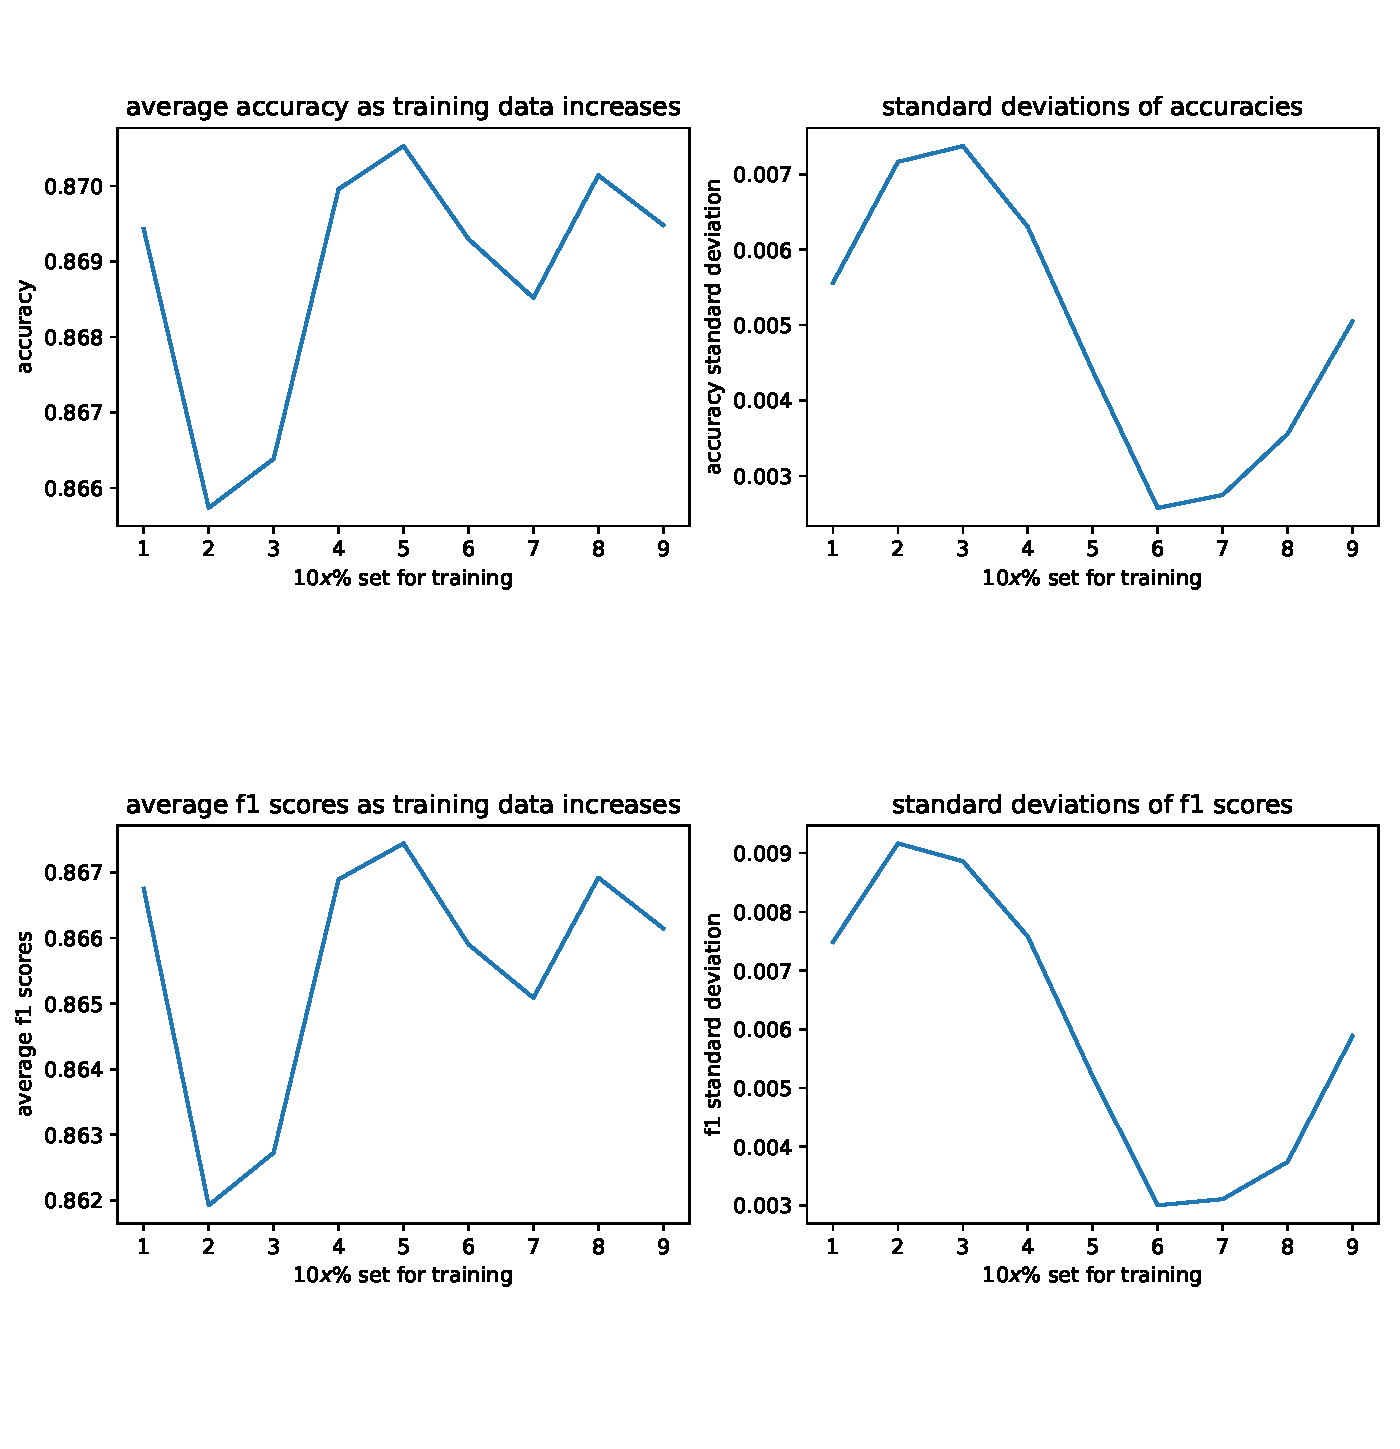
\includegraphics[width=0.6\textwidth]{img/Figure_3.pdf}
    \caption{Visual of averages and standard deviations as training size increases.}
    \label{fig:1}
\end{figure}

It can be seen that an increase in training size does provide slight improvments in average accuracies and f1 scores, however the standard deviations vary per trial run. Using Table \ref{tab:1} suggests that a training size of 60\% provides high averages for both accuracy and F1, with low standard deviations. This is indicative of a well-performing model, and could be used for further classifications.

Some potential limitations of this model may arise from the pruning of these unknown values as they potentially lose information, but in each experiment, keeping and removing these values, there was a general increase seen in the case where unknown values were removed.

\section{Conclusion}
Overall, this project aimed to provide a solidification of concepts learned so far in the course. Using data that provides a model with only slight improvements aids in ensuring critical thinking is used when working with these models. This ensures that when applying these concepts in real-world problems that we're not just ``pressing the button'', but rather understanding what it is we're trying to answer, and what is the best solution we can come up with to provide the best predictions.

\end{document}
